\documentclass[9pt,a4paper]{article}
\usepackage{amsfonts,amsmath,amsthm,amssymb,graphicx}
\usepackage{algorithm,algorithmicx,algpseudocode,subfigure}
\usepackage[utf8x]{inputenc}
\renewcommand\figurename{Figura}

\title{\bf Laborator 5}
\author{Sîrbu Matei-Dan}
\date{12 noiembrie 2020}

\begin{document}
\maketitle

\section*{Exercițiul 1}

\begin{figure}[htbp]
    \centering
    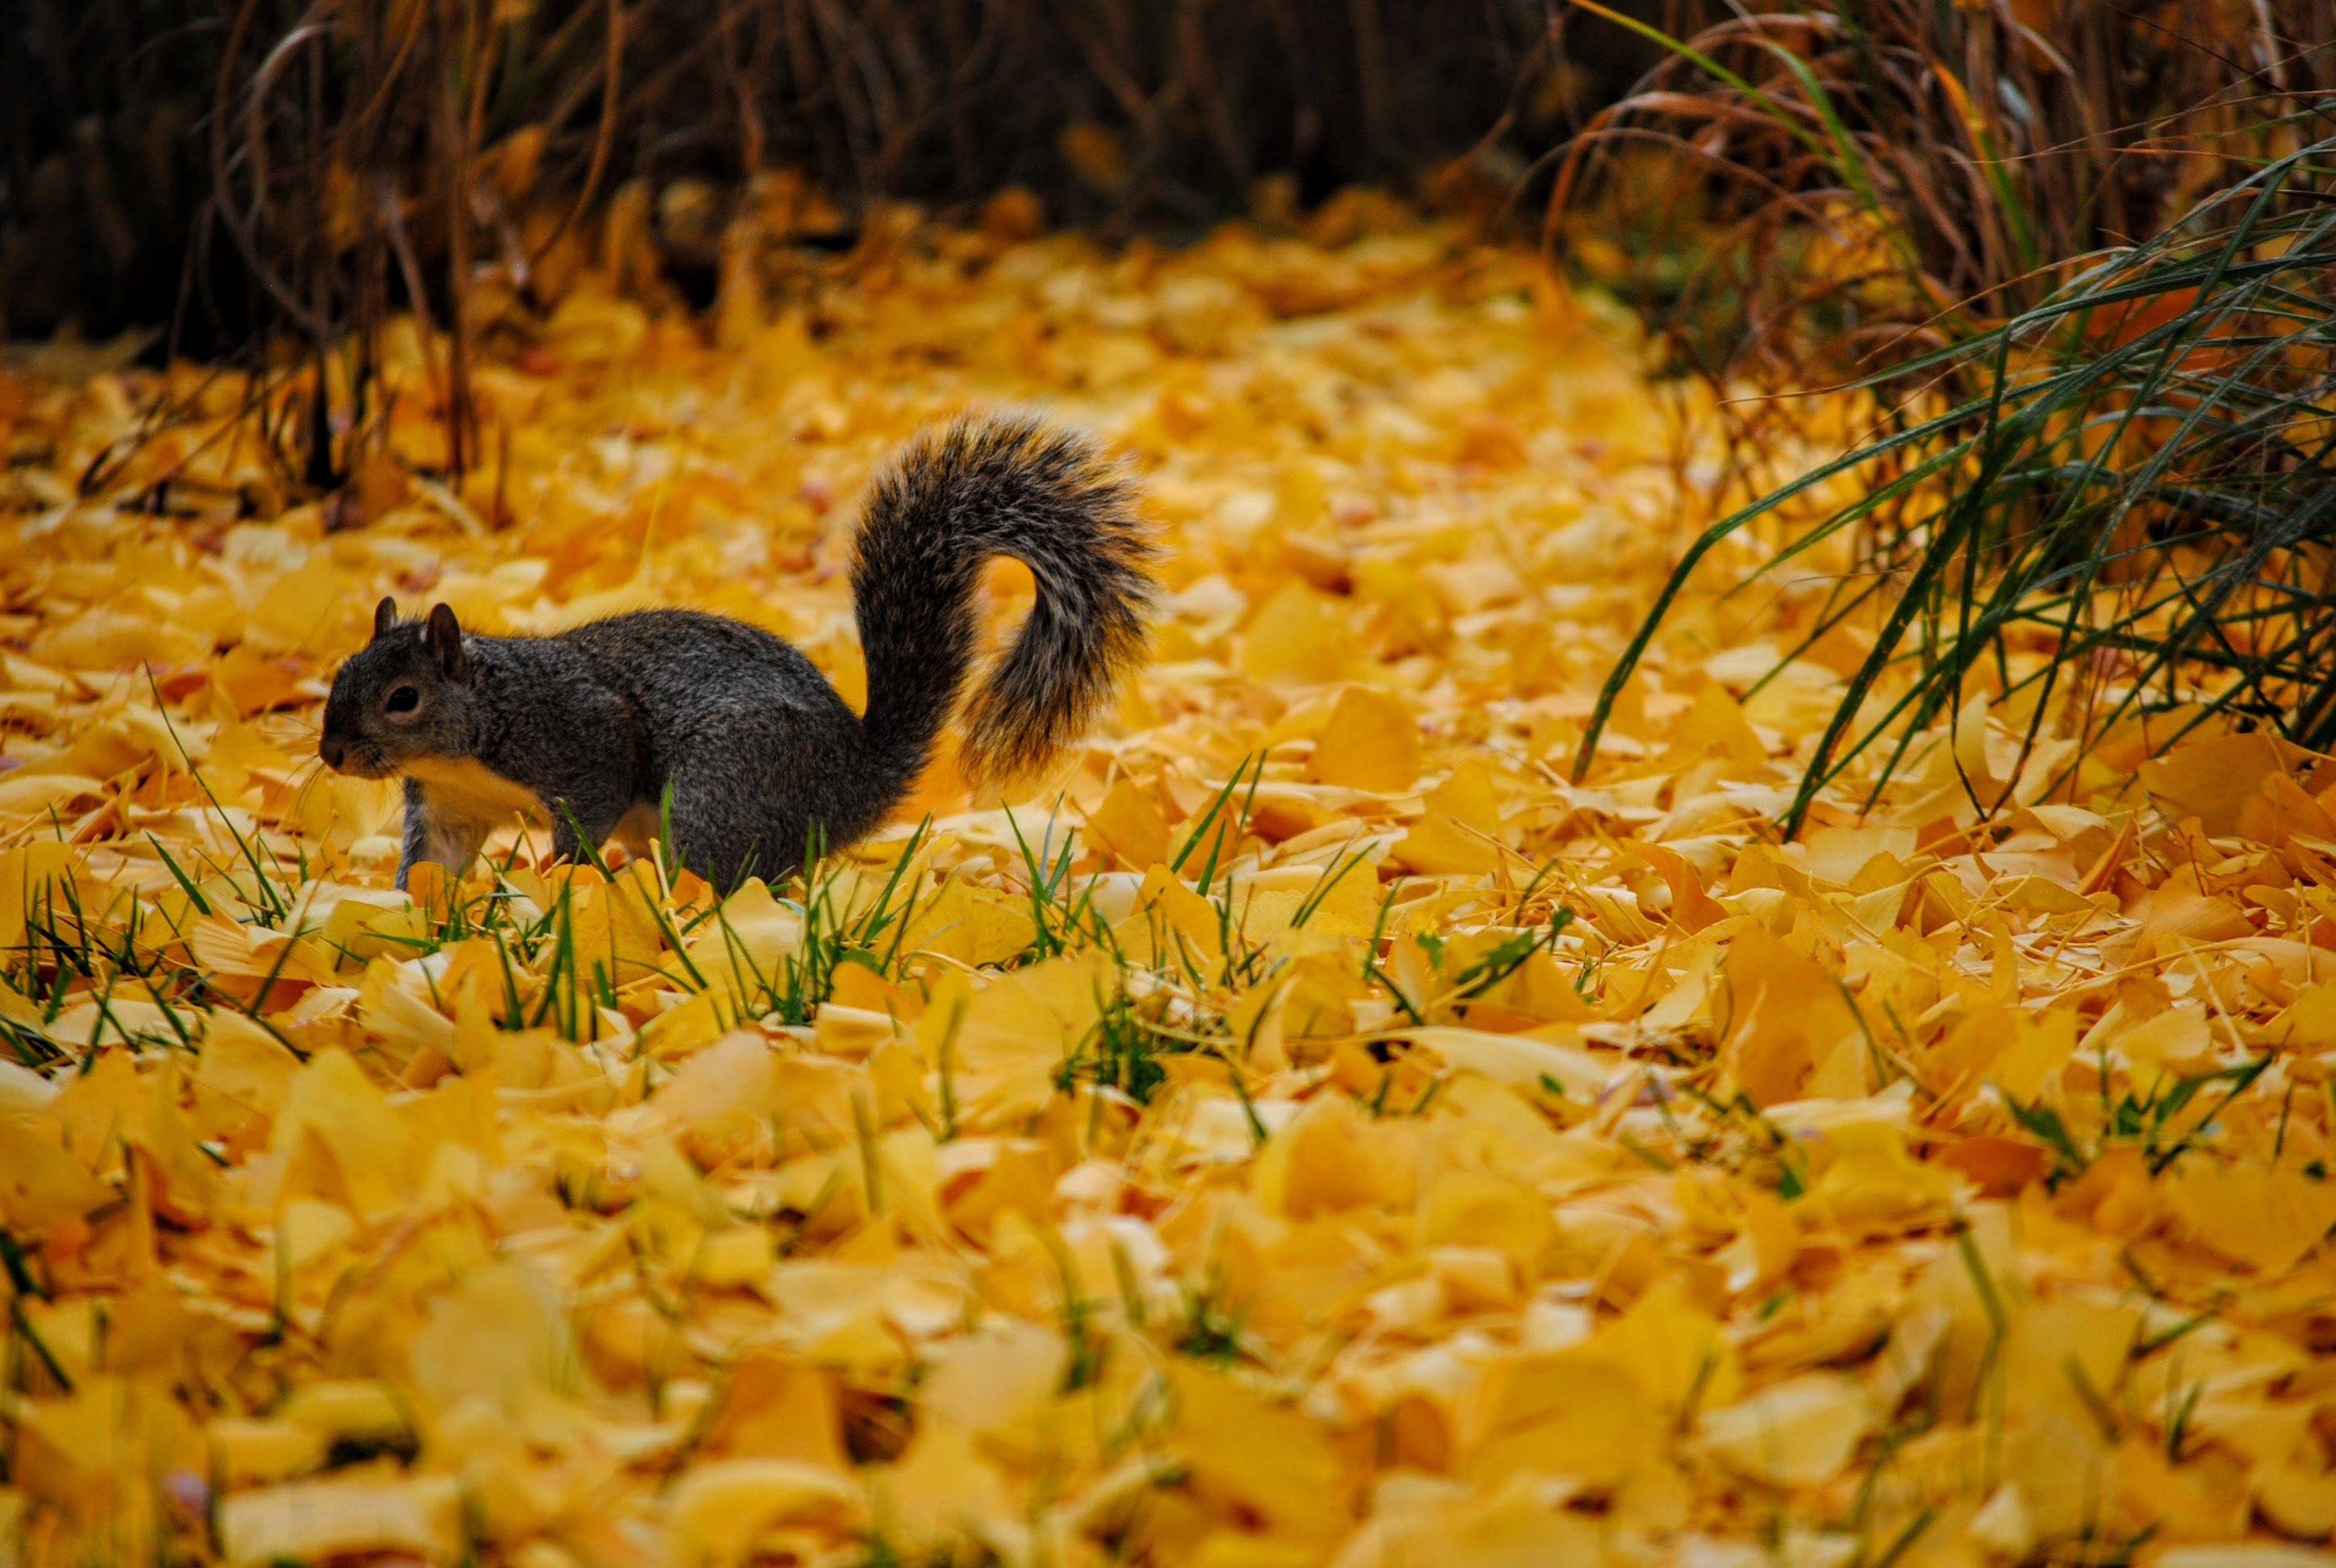
\includegraphics[trim= 10cm 20cm 50cm 15cm, clip, width=1\textwidth]{images/squirrel.jpg}
    \caption{Veveriță printre frunze}
\end{figure}

\begin{figure}[htbp]
    \centering
    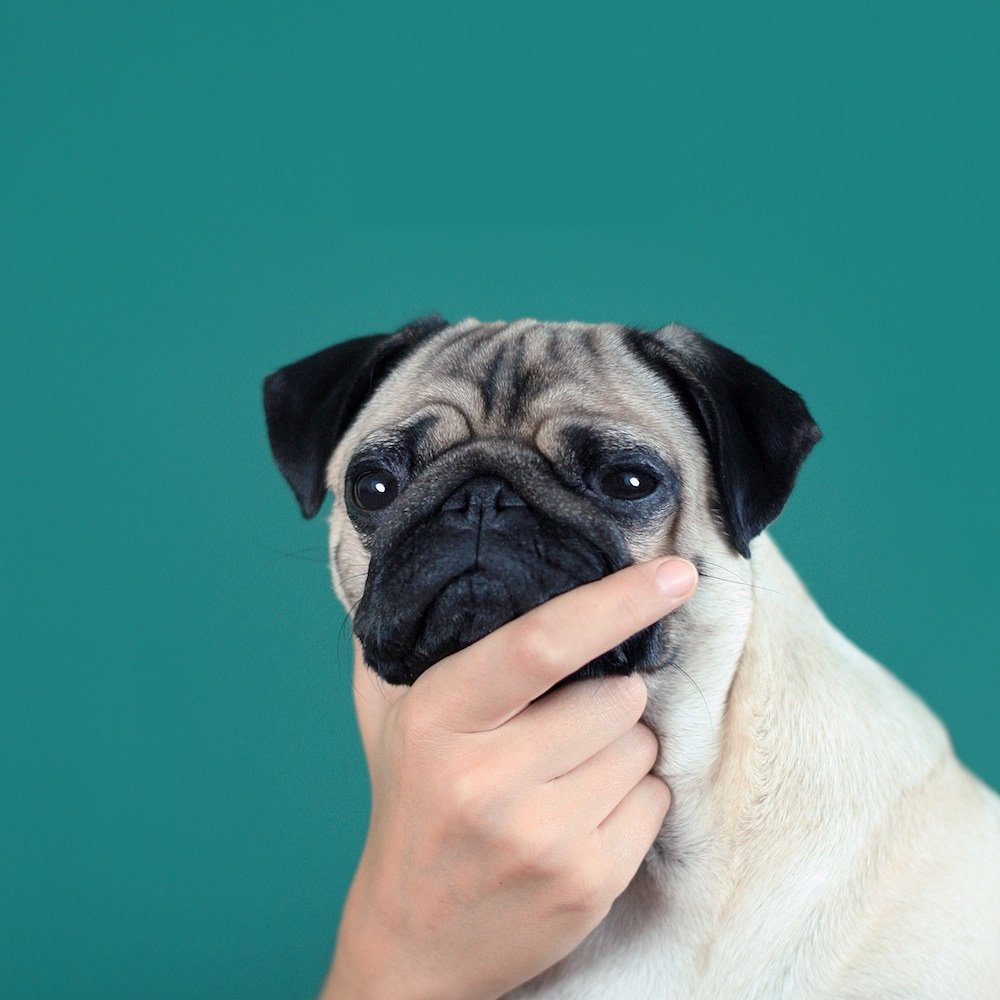
\includegraphics[trim= 10cm 10cm 0 12cm, clip, width=1\textwidth]{images/pug.jpg}
    \caption{Câine gânditor}
\end{figure}

\begin{figure}[htbp]
    \centering
    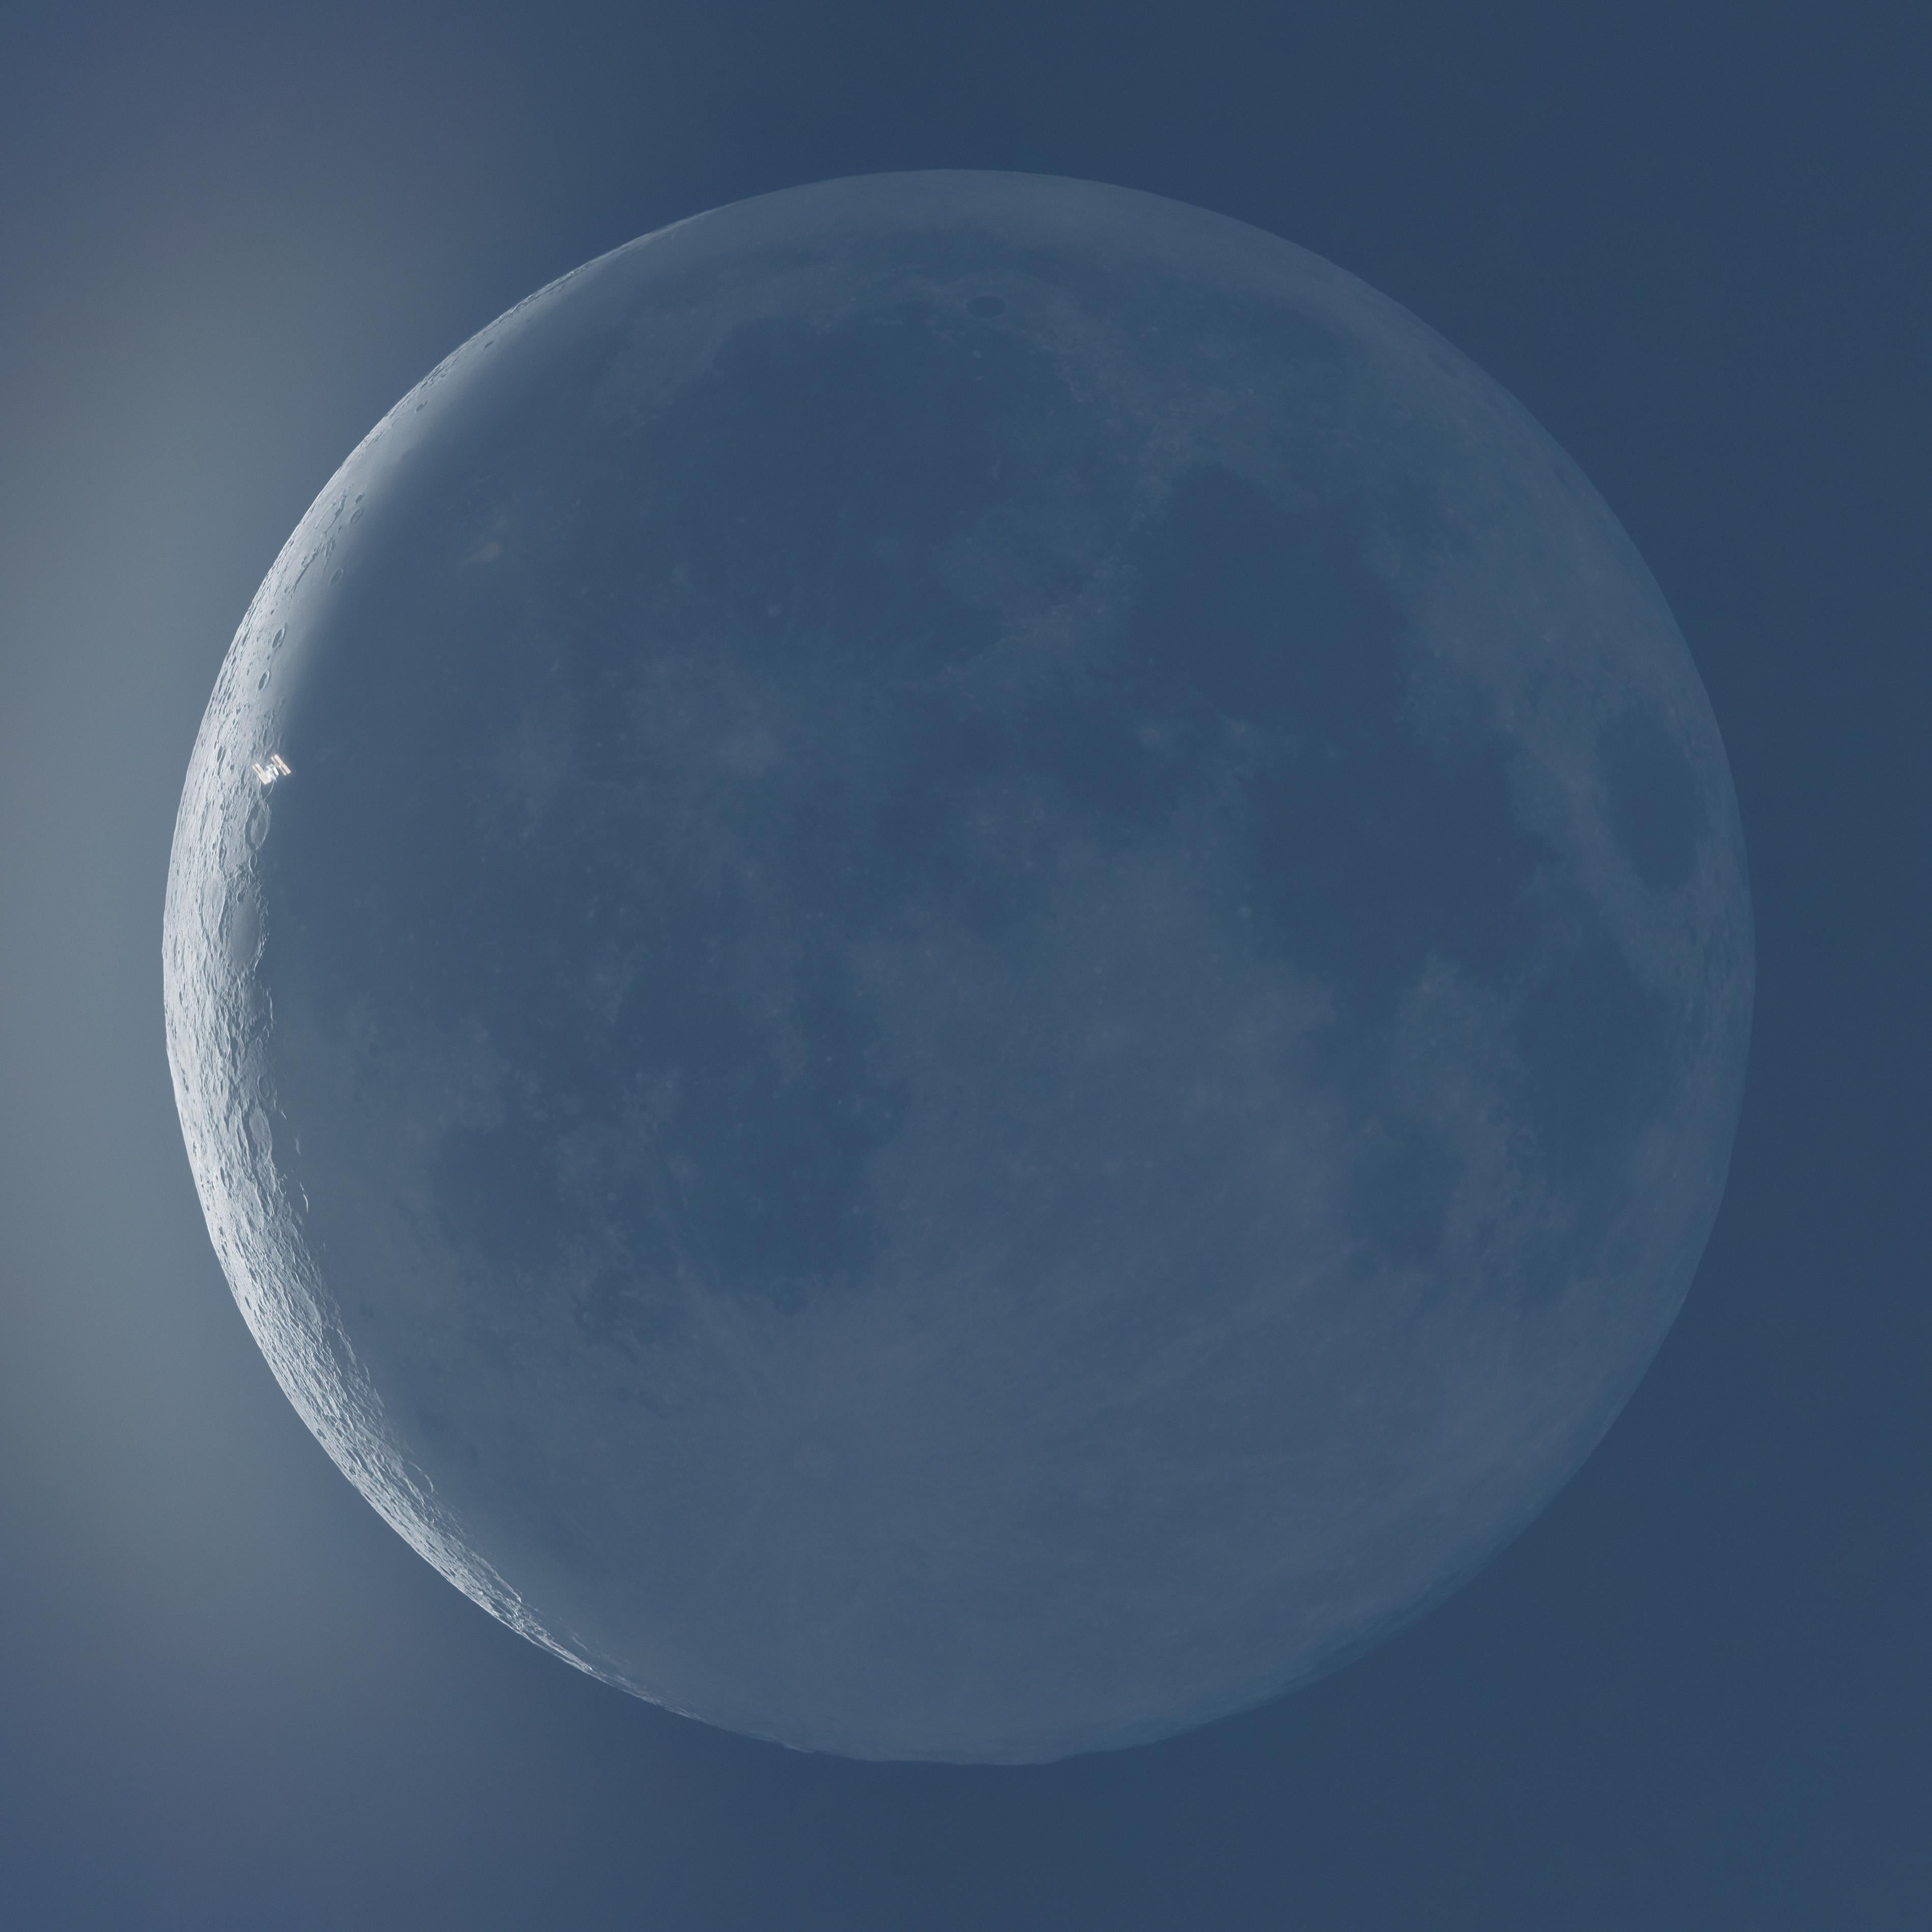
\includegraphics[trim= 0 50cm 80cm 40cm, clip, width=1\textwidth]{images/iss_transit.jpg}
    \caption{Stația Spațială Internațională tranzitând luna}
\end{figure}

\newpage

\begin{figure}[htbp]
    \centering
    \subfigure[Toamna 1]{\label{fig:autumn1}
        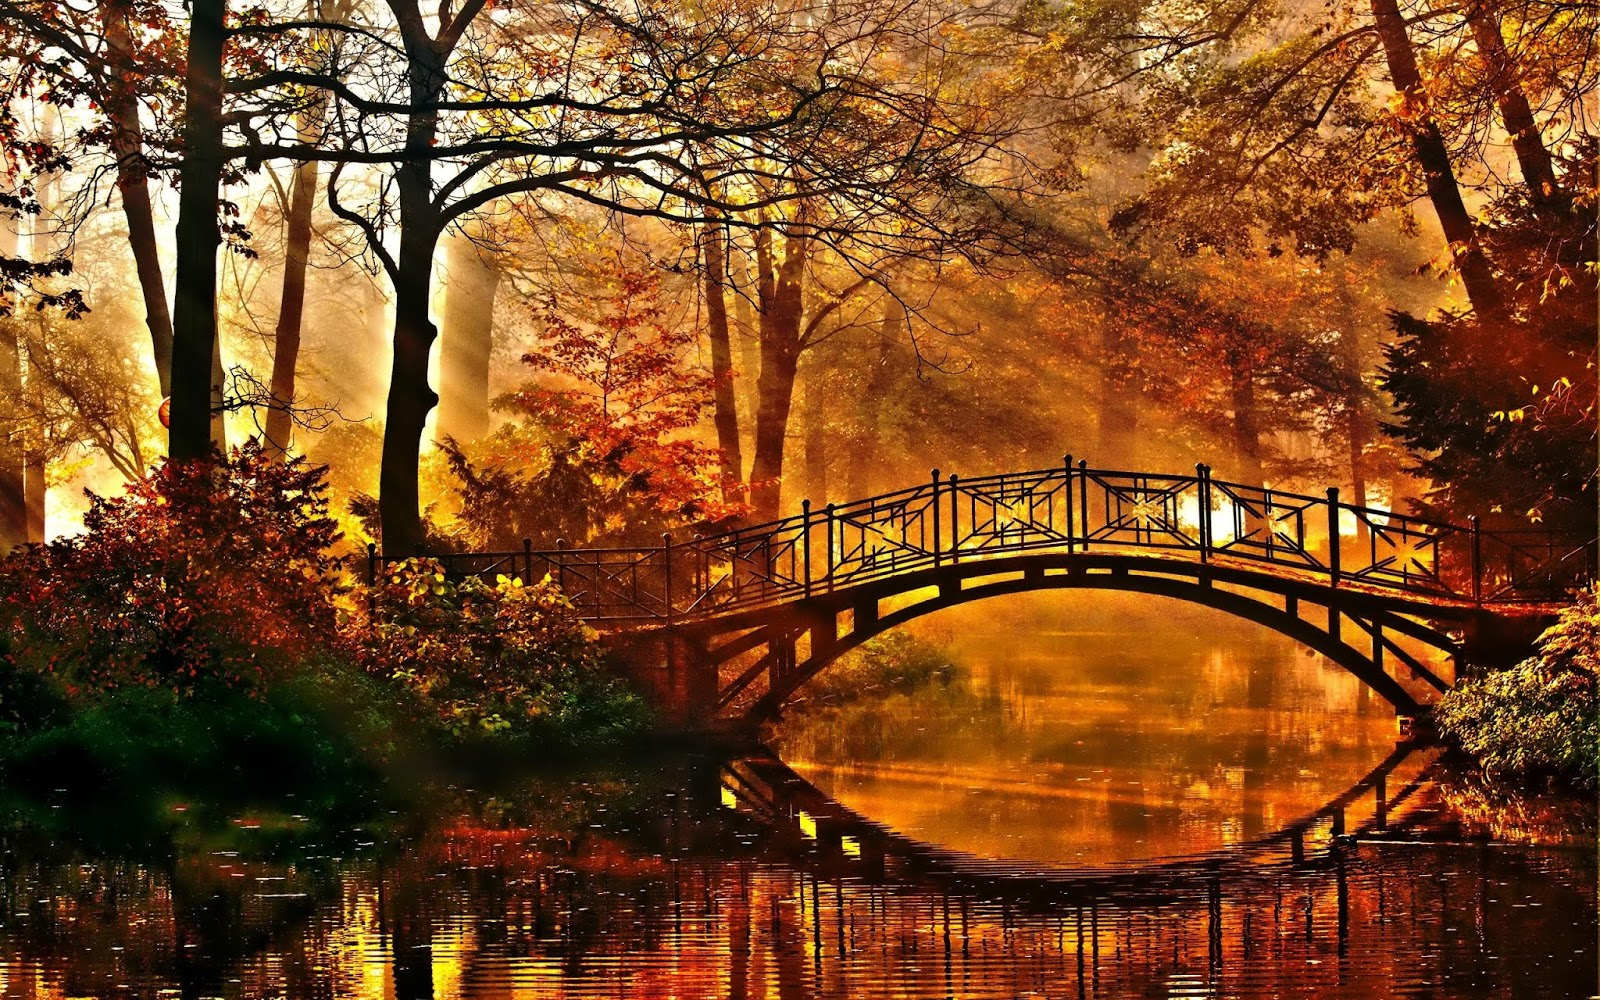
\includegraphics[width=0.3\textwidth]{images/bridge.jpg}}
    \subfigure[Toamna 2]{\label{fig:autumn2}
        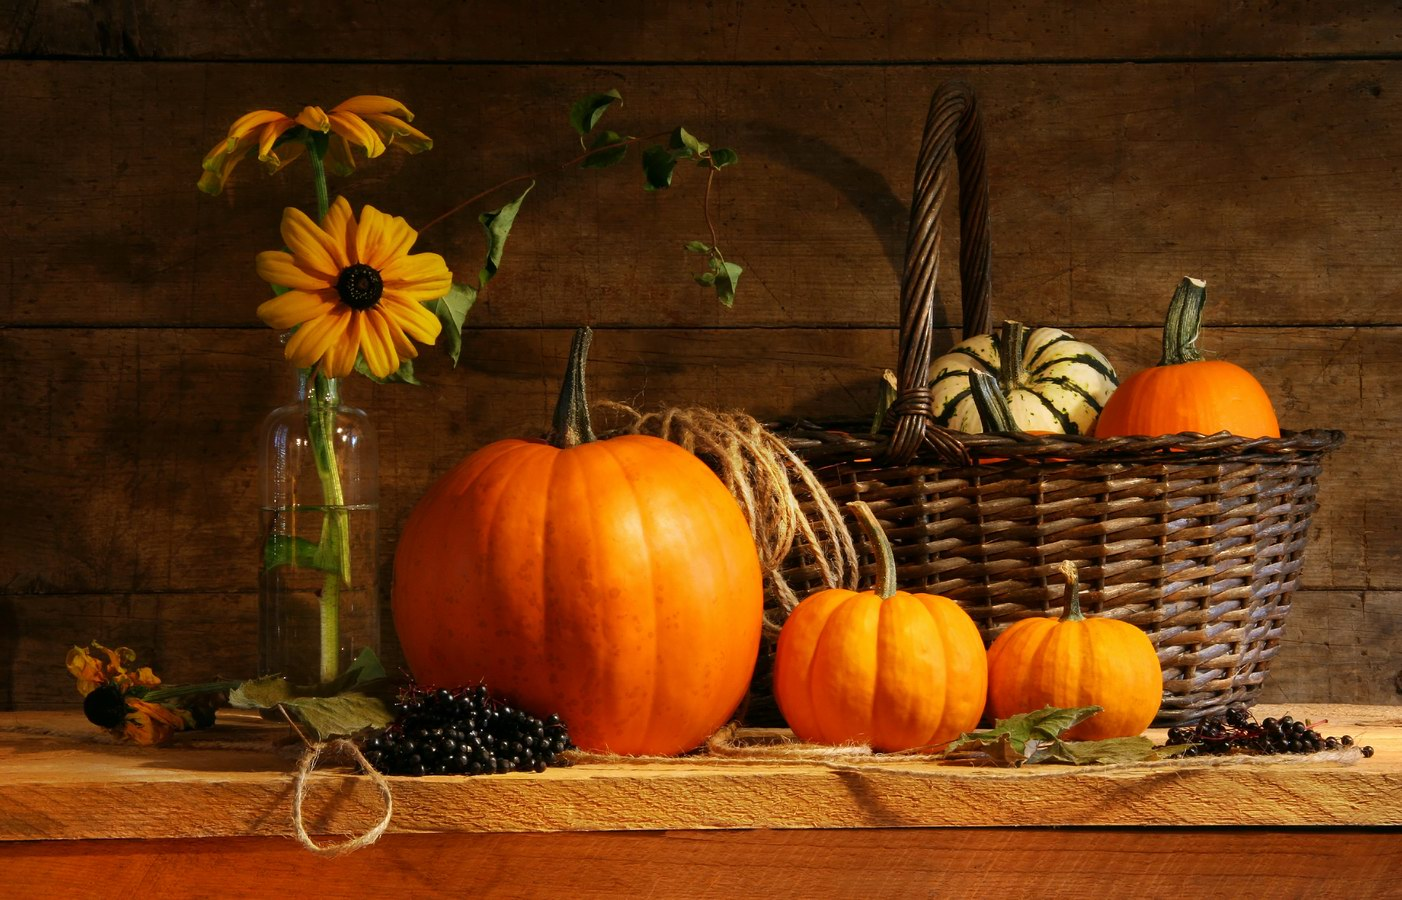
\includegraphics[width=0.3\textwidth]{images/pumpkin.jpg}}
    \subfigure[Toamna 3]{\label{fig:autumn3}
        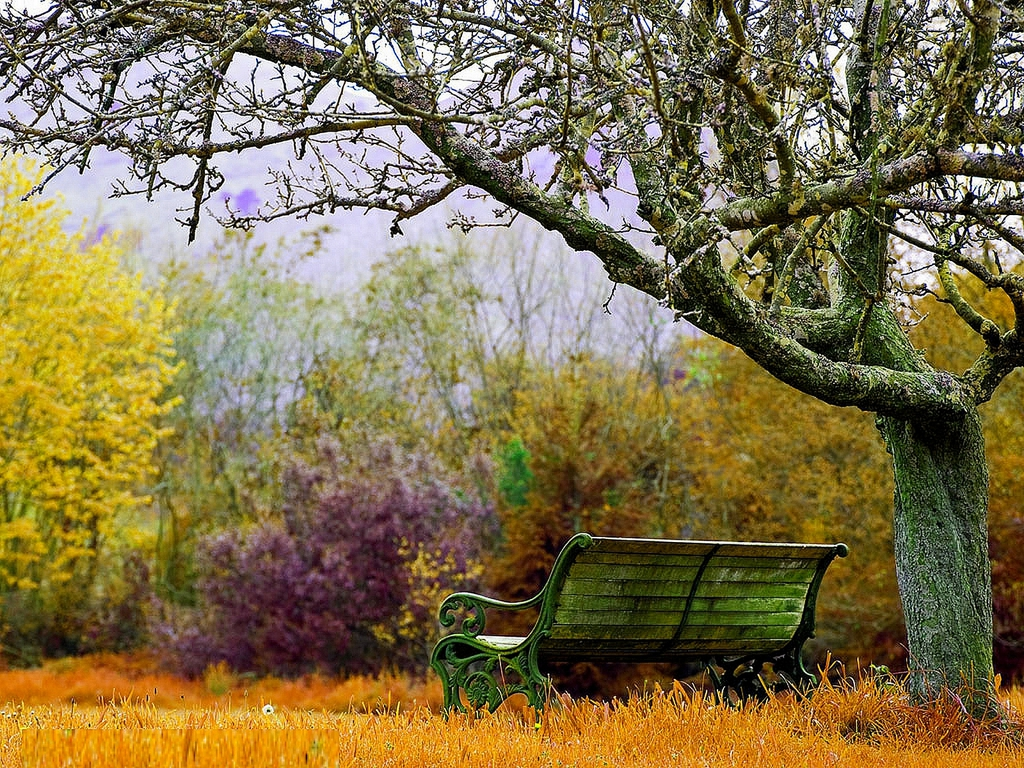
\includegraphics[width=0.3\textwidth, trim=0 0 0 4cm, clip]{images/bench.jpg}}
    \caption{Toamna}
    \label{fig:autumn}
\end{figure}

\section*{Exercițiul 2}
\subsection*{1. Algoritmi elementari de sortare}
\begin{algorithm}
    \begin{algorithmic}
        \Procedure{insert}{$T[1 \dots n]$}\Comment{Sortare prin inserție}
            \For{$i \gets 2$ \textbf{to} {$n$}}
                \State {$x \gets T[i]; j \gets i-1$}
                \While{$j > 0$ \textbf{and} $x < T[j]$}
                    \State{$T[j+1] \gets T[j]$}
                    \State{$j \gets j-1$}
                \EndWhile
                \State{$T[j+1] \gets x$}
            \EndFor
        \EndProcedure
        \\
        \Procedure{select}{$T[1 \dots n]$}\Comment{Sortare prin selecție}
            \For{$i \gets 1$ \textbf{to} {$n-1$}}
                \State{$minj \gets i; minx \gets T[i]$}
                \For{$j \gets i+1$ \textbf{to} {$n$}}
                    \If{$T[j] < minx$}
                        \State{$minj \gets j$}
                        \State{$minx \gets T[j]$}
                    \EndIf
                \EndFor
                \State{$T[minj] \gets T[i]$}
                \State{$T[i] \gets minx$}
            \EndFor
        \EndProcedure
    \end{algorithmic}
\end{algorithm}

\newpage

\subsection*{2. Algoritmul Greedy}
\begin{algorithm}
    \begin{algorithmic}
        \Procedure{greedy}{$C$}\Comment{$C$ este mulțimea candidaților}
            \State{$S \gets \varnothing$}\Comment{$S$ este mulțimea în care construim soluția}
            \While{\textbf{not} $\textsc{soluție}(S)$ \textbf{and} $C \neq \varnothing$}
                \State{$x \gets $ un element care maximizează \textsc{select}($x$)}
                \State{$C \gets C \backslash \{ x \}$}
                \If{$\textsc{fezabil}(S \cup \{ x \})$}
                    \State{$S \gets S \cup \{ x \}$}
                \EndIf
            \EndWhile
            \If{$\textsc{soluție}(S)$}
                \State{\Return $S$}
            \Else
                \State{\Return "nu există soluție"}
            \EndIf
        \EndProcedure
    \end{algorithmic}
\end{algorithm}

\subsection*{3. Algoritmul înmulțirii ,,a la russe''}
\begin{algorithm}
    \begin{algorithmic}
        \Procedure{russe}{$A, B$}
            \State{$\textbf{arrays }X, Y$}\Comment{Inițializare}
            \State{$X[1] \gets A;\  Y[1] \gets B$}
            \State{$i \gets 1$}\Comment{Se construiesc cele două coloane}
            \While{$X[i] > 1$}
                \State{$X[i+1] \gets X[i] \textbf{ div } 2$}\Comment{\textbf{div} reprezintă împărțirea întreagă}
                \State{$Y[i+1] \gets Y[i] + Y[i]$}
                \State{$i \gets i + 1$}\Comment{Adună numerele $Y[i]$ coresp. numerelor $X[i]$ impare}
            \EndWhile
            \State{$prod \gets 0$}
            \While{$i > 0$}
                \If{$X[i]$ este impar}
                    \State{$prod \gets prod + Y[i]$}
                \EndIf
                \State{$i \gets i - 1$}
            \EndWhile
            \State{\Return{$prod$}}
        \EndProcedure
    \end{algorithmic}
\end{algorithm}

\newpage

\subsection*{4. Algoritm pentru șirul Fibonacci}
\begin{algorithm}
    \begin{algorithmic}
        \Procedure{fib3}{$n$}
            \State{$i \gets 1;\  j \gets 0;\  k \gets 0;\  h \gets 1$}
            \While{$n > 0$}
                \If{$n$ este impar}
                    \State{$t \gets jh$}
                    \State{$j \gets ih + jk + t$}
                    \State{$i \gets ik + t$}
                \EndIf
                \State{$t \gets h^2$}
                \State{$h \gets 2kh + t$}
                \State{$k \gets k^2 + t$}
                \State{$n \gets n \textbf{ div } 2$}
            \EndWhile
            \State{\Return{$j$}}
        \EndProcedure
    \end{algorithmic}
\end{algorithm}

\end{document}